\documentclass{article}
\usepackage{listings}
\usepackage[utf8]{inputenc}
\usepackage{amsmath}
\usepackage{amsfonts}
\usepackage{amssymb}
\usepackage{polski}
\usepackage{indentfirst}
\usepackage{graphicx}
\usepackage{pdfpages}
\usepackage{gauss}
%script adding bars in matrix
\usepackage{etoolbox}
\makeatletter
\patchcmd\g@matrix
 {\vbox\bgroup}
 {\vbox\bgroup\normalbaselines}% restore the standard baselineskip
 {}{}
\makeatother

\newcommand{\BAR}{%
  \hspace{-\arraycolsep}%
  \strut\vrule % the `\vrule` is as high and deep as a strut
  \hspace{-\arraycolsep}%
}


\begin{document}
\title{Sprawozdanie - Metody numeryczne i optymailzacja}
\author{Jakub Andryszczak 259519,\\ Jakub Żak 244255,\\ Maciej Cierpisz 249163}
\date{}
\maketitle

\newpage
\tableofcontents
%Tutaj zaczyna się wstęp

\newpage
\section{Zadanie nr. 1}
Rozwiązać ręcznie i komputerowo metodą eliminacji Gaussa poniższy układ równań
liniowych. Znaleźć elementy podstawowe (pivots).

\begin{equation}
    \begin{cases}
      2u-v=0 \\
     -u+2v-w=0 \\
     -v+2w-z = 0 \\
     -w+2z=5
    \end{cases}\,.
\end{equation}

Do wykonania tego zadania rozpisano lewą stronę jako macierz 4x4 oraz wektor wynikowy 4x1. Zostały one połączone dzięki czemu otrzymano macierz rozszerzoną 4x5. Poniżej przedstawiono kolejno sposób wyliczania macierzy stosując do tego metodę eliminacji Gaussa.

\[
  \linespread{2}\selectfont
  \addtolength{\arraycolsep}{10pt}
 \begin{gmatrix}[b]
2 & -1 & 0 & 0 & \BAR & 0\\
-1 & 2 & -1 & 0 & \BAR & 0\\
0 & -1 & 2 &-1 & \BAR & 0\\
0 & 0 & -1 & 2 & \BAR & 5
 \rowops
 \add[\cdot \frac1{2}]01
 %\mult{3}{\cdot \left(-\frac2{29}\right)}

 \end{gmatrix}
\]
  Elementem podstawowym dla pierwszej kolumny znajduje się w pierwszej kolumnie i ma wartość 2
\[
  \linespread{2}\selectfont
  \addtolength{\arraycolsep}{10pt}
 \begin{gmatrix}[b]
2 & -1 & 0 & 0 & \BAR & 0\\
0 & \frac3{2} & -1 & 0 & \BAR & 0\\
0 & -1 & 2 &-1 & \BAR & 0\\
0 & 0 & -1 & 2 & \BAR & 5
 \rowops
 \add[\cdot \frac2{3}]12
 %\mult{3}{\cdot \left(-\frac2{29}\right)}

 \end{gmatrix}
\]

\[
  \centering
  \linespread{2}\selectfont
  \addtolength{\arraycolsep}{10pt}
 \begin{gmatrix}[b]
2 & -1 & 0 & 0 & \BAR & 0\\
0 & \frac3{2} & -1 & 0 & \BAR & 0\\
0 & 0 & \frac4{3} &-1 & \BAR & 0\\
0 & 0 & -1 & 2 & \BAR & 5
 \rowops
 \add[\cdot \frac3{4}]23
 %\mult{3}{\cdot \left(-\frac2{29}\right)}

 \end{gmatrix}
\]

\[
  \centering
  \linespread{2}\selectfont
  \addtolength{\arraycolsep}{10pt}
 \begin{gmatrix}[b]
2 & -1 & 0 & 0 & \BAR & 0\\
0 & \frac3{2} & -1 & 0 & \BAR & 0\\
0 & 0 & \frac4{3} &-1 & \BAR & 0\\
0 & 0 & 0 & \frac5{4} & \BAR & 5
 \rowops
 \mult{3}{\cdot \left(-\frac4{5}\right)}
 \add[]23
 \end{gmatrix}
\]
 Kolejnymi elementami podstawowymi są liczby 1.5 , 1.(3) i 1.25
\[
  \centering
  \linespread{2}\selectfont
  \addtolength{\arraycolsep}{10pt}
 \begin{gmatrix}[b]
2 & -1 & 0 & 0 & \BAR & 0\\
0 & \frac3{2} & -1 & 0 & \BAR & 0\\
0 & 0 & \frac4{3} & 0 & \BAR & 4\\
0 & 0 & 0 & 1 & \BAR & 4
 \end{gmatrix}
\]

\[
  \centering
  \linespread{2}\selectfont
  \addtolength{\arraycolsep}{10pt}
 \begin{gmatrix}[b]
2 & -1 & 0 & 0 & \BAR & 0\\
0 & \frac3{2} & 0 & 0 & \BAR & 3\\
0 & 0 & 1 & 0 & \BAR & 3\\
0 & 0 & 0 & 1 & \BAR & 4
 \end{gmatrix}
\]

\[
  \centering
  \linespread{2}\selectfont
  \addtolength{\arraycolsep}{10pt}
 \begin{gmatrix}[b]
2 & 0 & 0 & 0 & \BAR & 2\\
0 & 1 & 0 & 0 & \BAR & 2\\
0 & 0 & 1 & 0 & \BAR & 3\\
0 & 0 & 0 & 1 & \BAR & 4
 \end{gmatrix}
\]

\[
  \centering
  \linespread{2}\selectfont
  \addtolength{\arraycolsep}{10pt}
 \begin{gmatrix}[b]
1 & 0 & 0 & 0 & \BAR & 1\\
0 & 1 & 0 & 0 & \BAR & 2\\
0 & 0 & 1 & 0 & \BAR & 3\\
0 & 0 & 0 & 1 & \BAR & 4
 \end{gmatrix}
\]

Napisano kod w języku Python, który wykonuje eliminację Gaussa bez wyboru elementu podstawowego. Kod znajduje się poniżej.
\begin{center}
  (TUTAJ MA BYĆ KOD)
\end{center}


\section{Zadanie nr. 2}

Rozwiązać poniższy układ równań liniowych metodą eliminacji Gaussa z częściowym
wyborem element podstawowego:

\begin{equation}
  \begin{cases}
    x_{1}+x_{2}+x_{3}=1 \\
   x_{1}+x_{2}+2x_{3}=2 \\
   x_{1} + 2x_{2} +2x_{3}= 1 
  \end{cases}\,.
\end{equation}

Wyjaśnij dlaczego elimin. Gaussa bez wyboru elementu podstawowego nie działa poprawnie.

\[
  \centering
  \linespread{2}\selectfont
  \addtolength{\arraycolsep}{10pt}
 \begin{gmatrix}[b]
1 & 1 & 1 & \BAR & 1\\
1 & 1 & 2 & \BAR & 2\\
1 & 2 & 2 & \BAR & 1
\rowops
\add[-1]02
\add[-1]01
 \end{gmatrix}
\]

\[
  \centering
  \linespread{2}\selectfont
  \addtolength{\arraycolsep}{10pt}
 \begin{gmatrix}[b]
1 & 1 & 1 & \BAR & 1\\
0 & 0 & 1 & \BAR & 1\\
0 & 1 & 1 & \BAR & 0
\rowops
\swap12
 \end{gmatrix}
\]

\[
  \centering
  \linespread{2}\selectfont
  \addtolength{\arraycolsep}{10pt}
 \begin{gmatrix}[b]
1 & 1 & 1 & \BAR & 1\\
0 & 1 & 1 & \BAR & 0\\
0 & 0 & 1 & \BAR & 1
\rowops
\add[-1]21
\add[-1]20
 \end{gmatrix}
\]

\[
  \centering
  \linespread{2}\selectfont
  \addtolength{\arraycolsep}{10pt}
 \begin{gmatrix}[b]
1 & 1 & 0 & \BAR & 0\\
0 & 1 & 0 & \BAR & -1\\
0 & 0 & 1 & \BAR & 1
\rowops
\add[-1]10
 \end{gmatrix}
\]

\[
  \centering
  \linespread{2}\selectfont
  \addtolength{\arraycolsep}{10pt}
 \begin{gmatrix}[b]
1 & 0 & 0 & \BAR & 1\\
0 & 1 & 0 & \BAR & -1\\
0 & 0 & 1 & \BAR & 1
 \end{gmatrix}
\]

Wyjaśnienie dlaczego eliminacja Gaussa bez wyboru elementu podstawowego przedstawiona jest na przykładzie następnego zadania.
Kod różni się w małym stopniu od tego zaimplementowanego w poprzednim zadaniu. Zmiana polega na dodaniu linijek odpowiadających za wybór elementu. Przedstawiona została poniżej.
\begin{center}
  (LINIJKI WYBIERAJĄCE ELEMENT)
\end{center}

\section{Zadanie nr. 3}

Rozwiązać ręcznie układ równań liniowych:
\begin{equation}
  \begin{cases}
    0,0001x_{1}+x_{2}=1 \\
   x_{1}+x_{2}=2  
  \end{cases}\,.
\end{equation}
przy pomocy eliminacji Gaussa z i bez wyboru elementu podstawowego, zaokrąglając wyniki
obliczeń do trzech znaczących cyfr.

  Początkowo rozwiązano układ nie wybierając elementu podstawowego.

\[
  \centering
  \linespread{2}\selectfont
  \addtolength{\arraycolsep}{10pt}
 \begin{gmatrix}[b]
  -10^{-4} & 1 & \BAR & 1\\
  1 & 1 & \BAR & 2
\rowops
\add[10^4]01
 \end{gmatrix}
\]

\[
  \centering
  \linespread{2}\selectfont
  \addtolength{\arraycolsep}{10pt}
 \begin{gmatrix}[b]
  -10^{-4} & 1 & \BAR & 1\\
  0 & 10^4 & \BAR & 10^4
\rowops
\mult{0}{\cdot \left(-10^4\right)}
\mult{1}{\cdot \left(10^{-4}\right)}
\add[-1]10
 \end{gmatrix}
\]

Podczas sumowania wiersza drugiego zaokrąglono wyniki do trzech liczb znaczących.

\[
  \centering
  \linespread{2}\selectfont
  \addtolength{\arraycolsep}{10pt}
 \begin{gmatrix}[b]
  1 & 0 & \BAR & 0\\
  0 & 1 & \BAR & 1
 \end{gmatrix}
\]

Po przeliczeniu okazało się że wynik jest niepoprawny. Błąd powstaje w drugim równaniu. Podstawiając wartości, które wyszły powstaje równanie:
\begin{equation}
  1=2
\end{equation}
Co jest sprzeczne z prawdą.

W drugim przypadku wybierano element podstawowy co pozwoliło na otrzymanie innego wyniku.

\[
  \centering
  \linespread{2}\selectfont
  \addtolength{\arraycolsep}{10pt}
 \begin{gmatrix}[b]
  -10^{-4} & 1 & \BAR & 1\\
  1 & 1 & \BAR & 2
\rowops
\swap01
 \end{gmatrix}
\]

\[
  \centering
  \linespread{2}\selectfont
  \addtolength{\arraycolsep}{10pt}
 \begin{gmatrix}[b]
  1 & 1 & \BAR & 2\\
  -10^{-4} & 1 & \BAR & 1
 \end{gmatrix}
\]

\[
  \centering
  \linespread{2}\selectfont
  \addtolength{\arraycolsep}{10pt}
 \begin{gmatrix}[b]
  1 & 1 & \BAR & 2\\
  0 & 1 & \BAR & 1
 \end{gmatrix}
\]

\[
  \centering
  \linespread{2}\selectfont
  \addtolength{\arraycolsep}{10pt}
 \begin{gmatrix}[b]
  1 & 0 & \BAR & 1\\
  0 & 1 & \BAR & 1
 \end{gmatrix}
\]
Po podstawieniu wartości, które wyszły okazały się one poprawne dla tego układu równań.
\section{Zadanie nr. 4}
Rozwiązać komputerowo układ równań liniowych:
\begin{equation}
  \begin{cases}
    0,835x_{1}+0,667x_{2}=0,168 \\
   0,333x_{1}+0,266x_{2}=0,067  
  \end{cases}\,.
\end{equation}
Następnie, proszę zmienić (zaburzyć) wartość elementu 2 b z 0.067 na 0.066 i porównać rozwiązanie
z uzyskanym dla układu niezaburzonego. Wyjaśnij dlaczego nastąpiła tak znacząca
zmiana rozwiązania posługując się wskaźnikiem uwarunkowania macierzy systemowej.

  Do wykonania tego zadania wykorzystano algorytm eliminacji Gaussa napisany dla zadania drugiego, podstawiając odpowiednie wartości.
Dla pierwszego przypadku wektor wyjściowy miał wartości:
\begin{equation}
  x =
  \begin{gmatrix}[b]
    1\\
    -1
  \end{gmatrix}
\end{equation}
  W momencie wymiany wartości elementu b wektor wyjściowy prezentuje się następująco:
  \begin{equation}
    x =
    \begin{gmatrix}[b]
      -665,(9)\\
      833,(9)
    \end{gmatrix}
  \end{equation}

Ta dość spora zmiana jest związana ze wskaźnikiem uwarunkowania macierzy, który dla obu przypadków jest dosyć wysoki. Oznacza to, że problem jest źle uwarunkowany. Tego typu zagadnienia nie nadają się do numerycznego rozwiązania, ponieważ już sam błąd wynikający z numerycznej reprezentacji liczb wprowadza nieproporcjonalnie duży błąd w odpowiedzi.

\section{Zadanie nr. 5}
Zaimplementuj dowolny algorytm do faktoryzacji LU i zastosuj do macierzy:
\begin{equation}
  A=
  \begin{gmatrix}[b]
    1 & 2 & 3 & 4\\
    -1 & 1 & 2 & 1\\
    0 & 2 & 1 & 3\\
    0 & 0 & 1 & 1
  \end{gmatrix}
\end{equation}
Wyznacz det(A) na podstawie faktorów. Znajdź rozwiązanie dla układu równań Ax b dla b = $[1...1]^{T}$ , posługując się otrzymanymi faktorami.

Zdecydowano się na algorytm Crout. Poniżej implementacja algorytmu na zadanej macierzy.\\
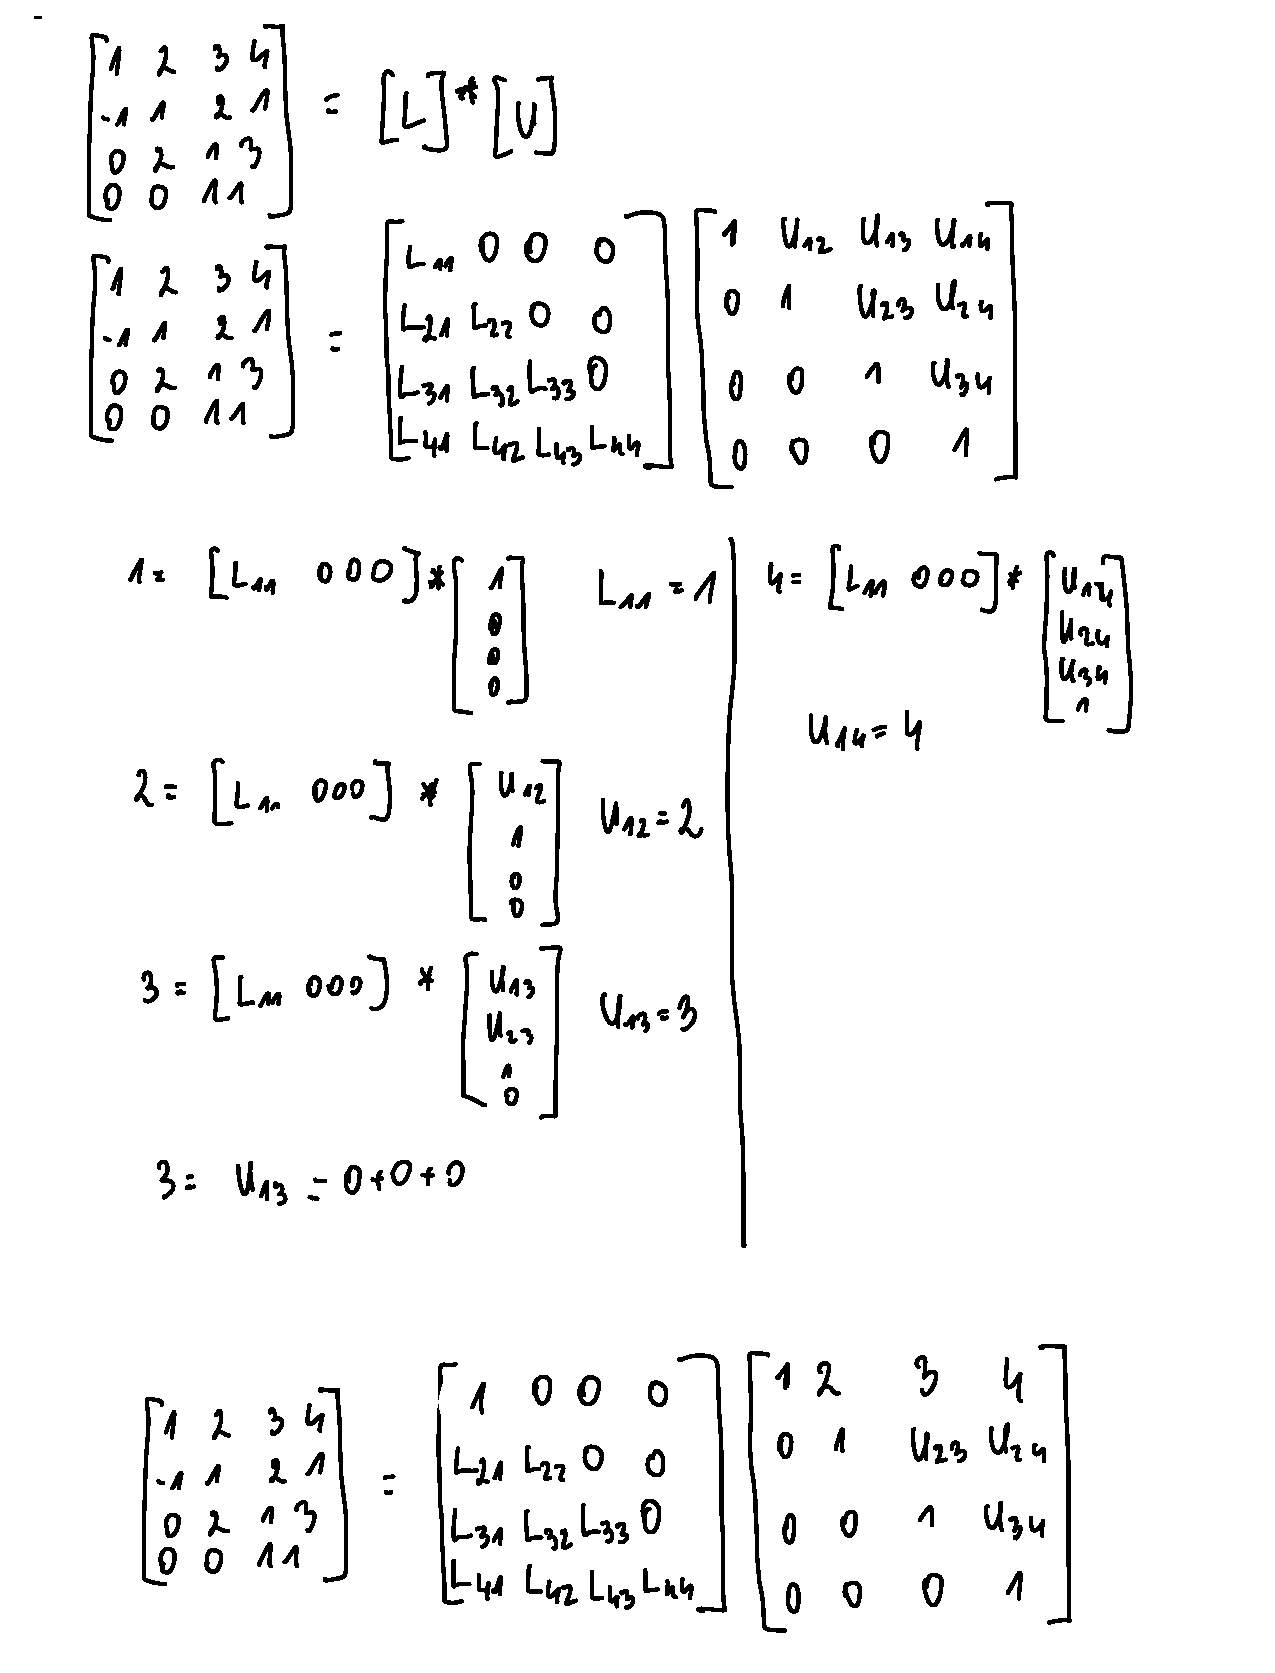
\includepdf[pages=-]{zad5.pdf}
\section{Zadanie nr. 6}
Przekształć ręcznie poniższą macierz do postaci RREF, wyznacz rank (A) oraz
wskaż kolumny odpowiadające zmiennym podstawowym i wolnym.

\begin{equation}
  A=
  \begin{gmatrix}[b]
  1 & 2 & 2 & 3 & 1\\
  2 & 4 & 4 & 6 & 2\\
  3 & 6 & 6 & 9 & 6\\
  1 & 2 & 4 & 5 & 3 
\end{gmatrix}
\end{equation}

Etapy rozwiązania macierzy przedstawiono poniżej:
\[
  \centering
  \linespread{2}\selectfont
  \addtolength{\arraycolsep}{10pt}
 \begin{gmatrix}[b]
  1 & 2 & 2 & 3 & 1\\
  2 & 4 & 4 & 6 & 2\\
  3 & 6 & 6 & 9 & 6\\
  1 & 2 & 4 & 5 & 3 
 \rowops
 \add[-2]01
 \add[-3]02
 \add[-1]03
\end{gmatrix}
\]
\[
  \centering
  \linespread{2}\selectfont
  \addtolength{\arraycolsep}{10pt}
 \begin{gmatrix}[b]
  1 & 2 & 2 & 3 & 1\\
  0 & 0 & 0 & 0 & 0\\
  0 & 0 & 0 & 0 & 3\\
  0 & 0 & 2 & 2 & 2 
 \rowops
 \swap13
\end{gmatrix}
\]
\[
  \centering
  \linespread{2}\selectfont
  \addtolength{\arraycolsep}{10pt}
 \begin{gmatrix}[b]
  1 & 2 & 2 & 3 & 1\\
  0 & 0 & 2 & 2 & 2\\
  0 & 0 & 0 & 0 & 3\\
  0 & 0 & 0 & 0 & 0
 \rowops
 \mult{1}{\cdot \left(\frac1{2}\right)}
 \mult{2}{\cdot \left(\frac1{3}\right)}
\end{gmatrix}
\]
\[
  \centering
  \linespread{2}\selectfont
  \addtolength{\arraycolsep}{10pt}
 \begin{gmatrix}[b]
  1 & 2 & 2 & 3 & 1\\
  0 & 0 & 1 & 1 & 1\\
  0 & 0 & 0 & 0 & 1\\
  0 & 0 & 0 & 0 & 0
 \rowops
\add[-2]10
\add20
\add[-1]21
\end{gmatrix}
\]
\[
  \centering
  \linespread{2}\selectfont
  \addtolength{\arraycolsep}{10pt}
 \begin{gmatrix}[b]
  1 & 2 & 0 & 1 & 0\\
  0 & 0 & 1 & 1 & 0\\
  0 & 0 & 0 & 0 & 1\\
  0 & 0 & 0 & 0 & 0
\end{gmatrix}
\]

Wartość rank(A) = 3, zmienne podstawowe ($A_{*1},A_{*3},A_{*5}$), zmienne wolne ($A_{*2},A_{*4}$)

\section{Zadanie nr. 7}
Zaimplementuj dowolną metodę ortogonalizacji macierzy i wyznacz faktoryzację
QR macierzy:
\begin{equation}
  A=
  \begin{gmatrix}[b]
  -2 & 1 & 2 & 1 \\
  2 & -1 & 2 & 1\\
  2 & 3 & -4 & 5\\
  2 & 3 & 0 & -1 
\end{gmatrix}
\end{equation}
place your code here

\section{Zadanie nr. 8}

Niech Ax = b , gdzie , symbol  oznacza iloczyn Kroneckera,
 jest macierzą jednostkową,  C jest macierzą losową wygenerowaną z rozkładu
równomiernego (rand), M = 200, N = 30, oraz   (rozkład normalny - randn).
Rozwiąż układ równań różnymi metodami bezpośrednimi (eliminacja Gaussa, faktoryzacja LU,
faktoryzacja QR) i porównaj metody ze względu na czas wykonywania się algorytmów i błąd
aproksymacji rozwiązania.



\section{Zadanie nr. 9}
Znajdź prądy gałęziowe zakładając, że wszystkie rezystancje wynoszą 20 Ohm.
równania
mpo

\[ \begin{bmatrix}
  \centering
  \linespread{2}\selectfont
  \addtolength{\arraycolsep}{10pt}
  0 & 0 & R & 0 & R & 0\\
  0 & 0 & -R & R & 0 & 0\\
  0 & 0 & 0 & 0 & R & -R\\
  -1 & 0 & 1 & 1 & 0 & 0\\
  0 & 1 & 1 & 0 & -1 & 0\\
  0 & 1 & 0 & -1 & 0 & 1\\

\end{bmatrix}
\times
\begin{bmatrix}
  I_{1}\\
  I_{2}\\ 
  I_{3}\\ 
  I_{4}\\ 
  I_{5}\\ 
  I_{6}\\ 
\end{bmatrix}
=
\begin{bmatrix}
  E_{1}\\
  E_{2}\\ 
  E_{3}\\ 
  0\\ 
  0\\ 
  0\\ 
\end{bmatrix} \]

\[
  \centering
  \linespread{2}\selectfont
  \addtolength{\arraycolsep}{10pt}
 \begin{gmatrix}[b]
  0 & 0 & 20 & 0 & 20 & 0 & \BAR & 20\\
  0 & 0 & -20 & 20 & 0 & 0 & \BAR & 10\\
  0 & 0 & 0 & 0 & 20 & -20 & \BAR & 10\\
  -1 & 0 & 1 & 1 & 0 & 0 & \BAR & 0\\
  0 & 1 & 1 & 0 & -1 & 0 & \BAR & 0\\
  0 & 1 & 0 & -1 & 0 & 1 & \BAR & 0
  \rowops
  \swap03
  \swap14
  \swap25
\end{gmatrix}
\]

\[
  \centering
  \linespread{2}\selectfont
  \addtolength{\arraycolsep}{10pt}
 \begin{gmatrix}[b]
  -1 & 0 & 1 & 1 & 0 & 0 & \BAR & 0\\
  0 & 1 & 1 & 0 & -1 & 0 & \BAR & 0\\
  0 & 1 & 0 & -1 & 0 & 1 & \BAR & 0\\
  0 & 0 & 20 & 0 & 20 & 0 & \BAR & 20\\
  0 & 0 & -20 & 20 & 0 & 0 & \BAR & 10\\
  0 & 0 & 0 & 0 & 20 & -20 & \BAR & 10
  \rowops
  \add[-1]12
\end{gmatrix}
\]

\[
  \centering
  \linespread{2}\selectfont
  \addtolength{\arraycolsep}{10pt}
 \begin{gmatrix}[b]
  -1 & 0 & 1 & 1 & 0 & 0 & \BAR & 0\\
  0 & 1 & 1 & 0 & -1 & 0 & \BAR & 0\\
  0 & 0 & -1 & -1 & 1 & 1 & \BAR & 0\\
  0 & 0 & 20 & 0 & 20 & 0 & \BAR & 20\\
  0 & 0 & -20 & 20 & 0 & 0 & \BAR & 10\\
  0 & 0 & 0 & 0 & 20 & -20 & \BAR & 10
  \rowops
  \add[20]23
  \add[-20]24
\end{gmatrix}
\]

\[
  \centering
  \linespread{2}\selectfont
  \addtolength{\arraycolsep}{10pt}
 \begin{gmatrix}[b]
  -1 & 0 & 1 & 1 & 0 & 0 & \BAR & 0\\
  0 & 1 & 1 & 0 & -1 & 0 & \BAR & 0\\
  0 & 0 & -1 & -1 & 1 & 1 & \BAR & 0\\
  0 & 0 & 0 & -20 & 40 & 20 & \BAR & 20\\
  0 & 0 & 0 & 40 & -20 & -20 & \BAR & 10\\
  0 & 0 & 0 & 0 & 20 & -20 & \BAR & 10
  \rowops
  \add[2]34
\end{gmatrix}
\]

\[
  \centering
  \linespread{2}\selectfont
  \addtolength{\arraycolsep}{10pt}
 \begin{gmatrix}[b]
  -1 & 0 & 1 & 1 & 0 & 0 & \BAR & 0\\
  0 & 1 & 1 & 0 & -1 & 0 & \BAR & 0\\
  0 & 0 & -1 & -1 & 1 & 1 & \BAR & 0\\
  0 & 0 & 0 & -20 & 40 & 20 & \BAR & 20\\
  0 & 0 & 0 & 0 & 60 & 20 & \BAR & 50\\
  0 & 0 & 0 & 0 & 20 & -20 & \BAR & 10
  \rowops
  \add[-\frac1{3}]45
\end{gmatrix}
\]

\[
  \centering
  \linespread{2}\selectfont
  \addtolength{\arraycolsep}{10pt}
 \begin{gmatrix}[b]
  -1 & 0 & 1 & 1 & 0 & 0 & \BAR & 0\\
  0 & 1 & 1 & 0 & -1 & 0 & \BAR & 0\\
  0 & 0 & -1 & -1 & 1 & 1 & \BAR & 0\\
  0 & 0 & 0 & -20 & 40 & 20 & \BAR & 20\\
  0 & 0 & 0 & 0 & 60 & 20 & \BAR & 50\\
  0 & 0 & 0 & 0 & 0 & -\frac{80}{3} & \BAR & -\frac{20}{3}
\end{gmatrix}
\]

tego typu benc benc

\section{Wnioski}
Zgodnie z obliczeniami wyniki obliczeń zostały wykonane prawidłowo
\end{document} 